\section{Basic Application}\label{TM:sec:basic}
The basic operation of the thermal model is performed via the MATLAB command-line using two functions: \texttt{xls\_prep.m} and \texttt{thermal.m} (the source code is included in Section \ref{TM:sec:source}).  These two functions were utilized by \texttt{saMODEL2.m} as detailed in Appendix \ref{apx:sobol}.  First, \texttt{xls\_prep.m} is implemented, which requires three input arrays that contain the snow properties, atmospheric conditions, and model constants.  The syntax for \texttt{xls\_prep.m} is as follows:

\begin{singlespaced}\begin{lstlisting}[style=inline]
function [s,a] = xls_prep(snow,atm,constants)
% XLS_PREP builds arrays for inputing into thermal model
%__________________________________________________________________________
% SYNTAX:
%   [snow,atm] = prep_input(snow,atm,constants);
\end{lstlisting}\end{singlespaced}

The \texttt{snow} variable may be arranged in two ways: as a uniform or a varying snowpack.  If the snowpack is assumed uniform then \texttt{snow} is a 1-D array with six values (in order): depth (cm), density (kg/m\spr{3}), thermal conductivity (W/(m$\cdot$K)), specific heat capacity (J/(gm$\cdot$K)), snow temperature (\C), and extinction coefficient (1/m).  If the snowpack varies then the array may be composed of any number of rows of the same parameters that dictates the different layers.  The following MATLAB code provides example definitions of the \texttt{snow} variable:
\begin{singlespaced}\begin{lstlisting}[style=inline]
>> snow = [50, 130, 0.06, 2030, -10, 70]
snow =
		50  130  0.06  2030  -10  70
>> snow = [0, 130, 0.06, 2030, -10, 70; 50, 180, 0.1, 2030, -5, 90;...
 100, 180, 0.1, 2030, -5, 90]
snow =
	0  130  0.06  2030  -10  70
	50  180  0.1  2030  -5  90
	100  180  0.1  2030  -5  90
>> 
\end{lstlisting}\end{singlespaced}

The first example defines a 50 cm thick snow pack with constant properties.  The second example defines a 100 cm deep snowpack that increases in density, thermal conductivity, temperature, and extinction coefficient from 0 to 50 cm.  Then from 50 to 100 cm the conditions remain constant.  The \texttt{xls\_prep.m} function performs linear interpolation between the rows according to the layer thickness.  An additional seventh column is optional that specifies the extinction coefficient for the near-infrared wavebands, in this case the extinction coefficient previously mentioned is used for the visible waveband.

In similar fashion, the atmospheric conditions are defined in the \texttt{atm} variable, which includes nine parameters (in order): time (hours), incoming long-wave radiation (W/m\spr{2}), incoming short-wave radiation (W/m\spr{2}), albedo, wind speed (m/s), air temperature (\C), relative humidity (\%), the lower boundary condition (\C), and air pressure (kPa).  Two additional columns may also be defined that specifiy the incoming short-wave radiation and albedo for the near-infrared wavebands.  Again, the short-wave radiation and albedo previously defined are then used as the values for the visible spectrum.

The model constants are defined in the \texttt{constants} variable, which must include the following (in order): latent heat of sublimation (kJ/kg), the latent heat transfer coefficient, the sensible heat transfer coefficient, the ratio of molecular weights of dry-air and water-vapor, the gas constant for water-vapor (kJ/(kg$\cdot$K)), reference temperature (\C), reference vapor-pressure (kPa), the emissivity of snow, the layer thickness (cm), and time step (s).

Once the three input variable arrays are defined the thermal model may be executed, for example:
\begin{singlespaced}\begin{lstlisting}[style=inline]
>> snow = [50, 130, 0.06, 2030, -10, 70];
>> atm = [0,240,0,0.82,1.7,-10,.2,-10,101; 10,240,500,0.82,1.7,-10,.2,-10,101];
>> contants = [2833,0.0023,0.0023,0.622,0.462,-5,0.402,0.95,1,60,1];
>> [S,A] = xls_prep(snow, atm, constants);
>> [T,Q] = thermal(S, A, constants); 
\end{lstlisting}\end{singlespaced}

The \texttt{thermal.m} function implements the finite-difference solution presented in Chapter \ref{chapter5}.  This function outputs an array containing snow temperatures (\texttt{T}) as a function of model evaluation time (columns) and depth (rows).  The various heat-fluxes---long-wave, sensible, latent, short-wave---are output in the \texttt{Q} variable in similar fashion.

\section{Spreadsheet Application}\label{TM:sec:spread}
\subsection{General Application}
To make the thermal model more powerful, two additional functions were developed---\texttt{xls\_input.m} and \texttt{runmodel.m}---that provide an interface between MATLAB and Microsoft Excel. This allows the various input matrices previously explained to be easily developed. First, the required structure of the Excel file must be established.  The Excel spreadsheet must be composed of three worksheets named ``SnowProperties'', ``AtmosphericSettings'', and ``Constants''.  Each worksheet must be formatted in a specific fashion, as shown in Figures \ref{TM:fig:snowatm} and Figures \ref{TM:fig:constants}.\footnote{A template may be downloaded at: \href{http://www.coe.montana.edu/ce/subzero/snow/thermalmodel/template.xlsx}{\nolinkurl{www.coe.montana.edu/ce/subzero/snow/thermalmodel/template.xlsx}}.}  Section \secref{TM:sec:features} details some additional features available when using \texttt{xls\_input.m}, particularly for the ``Constants'' worksheet.  

\begin{figure}[ht!]\centering
\subfloat[Snow Properties]{\includegraphics[width=\linewidth]{\cfolder /figures/snow.png}}\\
\subfloat[Atmospheric Settings]{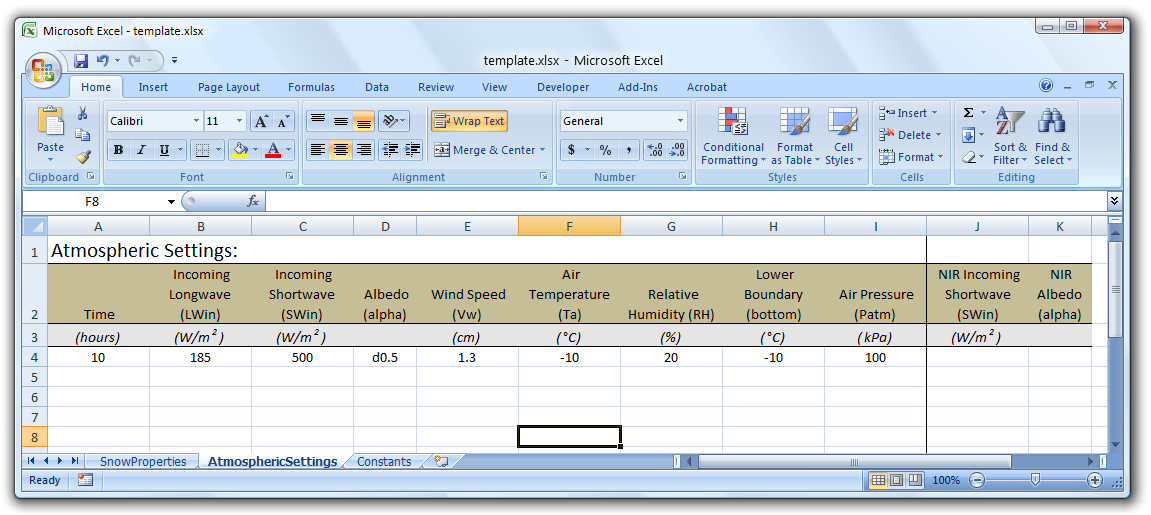
\includegraphics[width=\linewidth]{\cfolder /figures/atm.png}}\\
\caption{Example of the (a) ``SnowProperties'' and  (b)``AtmosphericSettings'' worksheets for Excel file read by \texttt{xls\_input.m}.}
\label{TM:fig:snowatm}
\end{figure}

\begin{figure}[b!]\centering
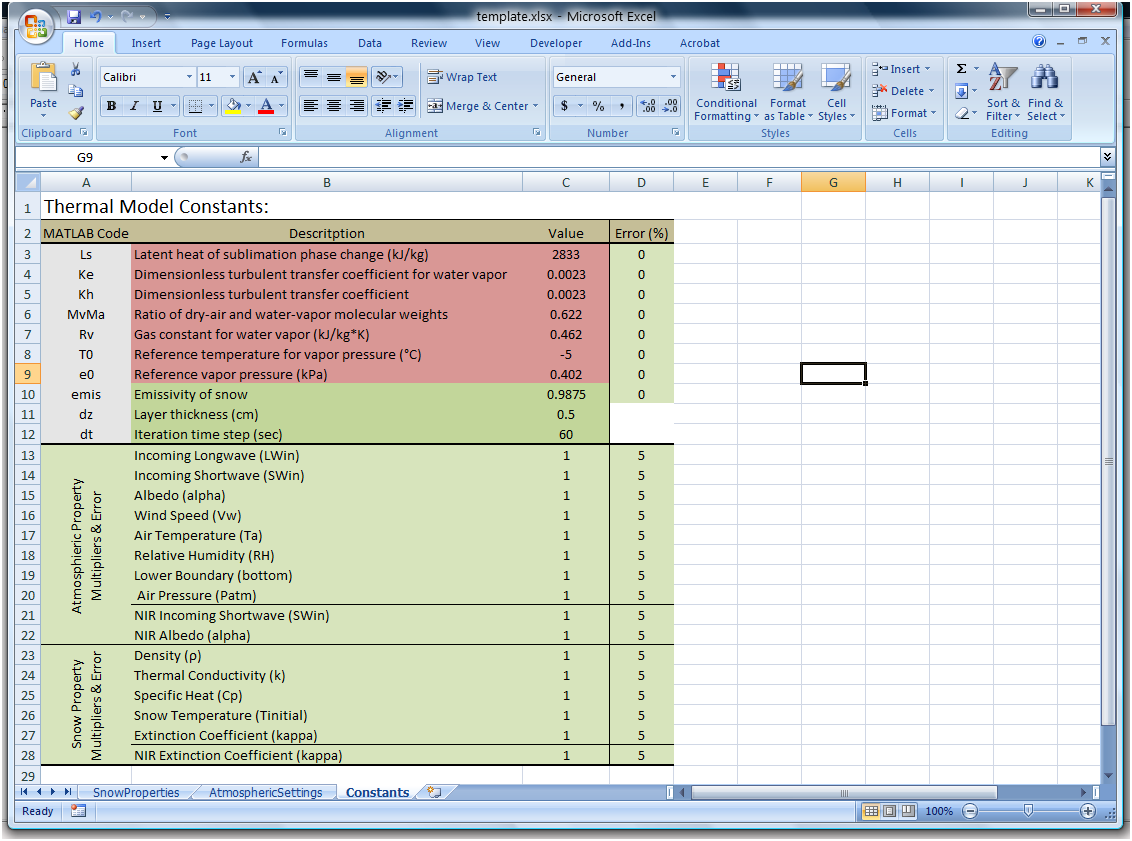
\includegraphics[width=\linewidth]{\cfolder /figures/constants.png}
\caption{Example of the ``Constants'' worksheets for Excel file read by \texttt{xls\_input.m}.}
\label{TM:fig:constants}
\end{figure}

Once the Excel file is setup as desired, the function \texttt{xls\_input.m} is used to process the data contained in the spreadsheet. As was the case for the basic operation, the near-infrared columns are optional.  For example, for the template.xlsx file available for download, the following code implements the thermal model:
\begin{singlespaced}\begin{lstlisting}[style=inline]
>> filename = 'template.xlsx';
>> [s,a,c] = xls_input(filename);
>> [S,A] = xls_prep(s, a, c);
>> [T,Q] = thermal(S, A, c); 
\end{lstlisting}\end{singlespaced}

The \texttt{runmodel.m} function performs the above actions, groups the results into a data structure, and adds the ability to compute confidence level intervals for the snow temperatures.  The confidence intervals are explained further in the following section.  The code shown in Figure \ref{TM:fig:runmodel} implements the thermal model via \texttt{runmodel.m} and displays the data structure produced.  The data structure and details regarding various optional inputs are explained in the help associated with the \texttt{runmodel.m}.  The data structure was designed to be implemented via the graphical user interface (Section \secref{TM:sec:gui}), as such the data structure may contain many model runs, as shown in Figure \ref{TM:fig:runmodel}.

\begin{figure}[ht!]
\begin{singlespaced}\begin{lstlisting}[style=figure]
>> filename = 'template.xlsx';
>> data = runmodel(filename)
data = 
             xls: 'template.xlsx'
    bootsettings: []
            name: ''
            desc: ''
            time: '22-Mar-2010 09:58:06'
               T: [82x601 double]
               Q: [81x601x5 double]
             snw: [81x7 double]
             atm: [601x11 double]
           const: [1x10 double]
           Tboot: []
           Qboot: []
           Sboot: []
           Aboot: []
           Cboot: []
>> data(2) = runmodel(filename); % multiple runs may be stored
>> 
\end{lstlisting}\end{singlespaced}
\caption{MATLAB implementation of \texttt{runmodel.m} and the resulting data structure.}
\label{TM:fig:runmodel}
\end{figure}

\subsection{Additional Features}\label{TM:sec:features}
The usage of the function \texttt{xls\_input.m} offers additional functionality for inputs, including the usage of tabulated snow micro-structure data, input multipliers, and confidence interval calculations.

\subsubsection{Snow Micro-Structure} The snow albedo and extinction coefficient may be input into the Excel document using keys: \emph{dXX}, \emph{classX}, or \emph{type}.\footnote{The \emph{italicized} keys are used to reference the inputs, the actual text as would be entered in the Excel worksheets is provide in quotes.}  The \emph{dXX} key allows the snow grain diameter to be used to compute albedo and extinction coefficient according to \citet[Eq. 2.25, p. 56]{armstrong2008}, were the \emph{XX} is a number representing the size of the grain in millimeters (e.g., \q{d5}).  Figure \ref{TM:fig:snowatm}b includes the implementation of this option. The \emph{classX} key uses the tabulated values from \citet[Tab. 2.6]{armstrong2008}, where \emph{X} is a value one to six (e.g., \q{class2}).  The type may be one of three strings: ``fine'', ``medium'', or ``coarse'', this option is only available for the computation of albedo.  The usage of these keys results in the computation of the albedo from the information provided in \citet{baldridge2009}.  The albedo and extinction coefficient calculations are preformed in the \texttt{albedo} and \texttt{extinction} sub-functions of \texttt{xls\_input.m}.

In all cases, when the optional near-infrared columns are not utilized it is assumed that albedo and extinction coefficients are defined for the ``all-wave'' spectrum that includes both the visible and near-infrared spectrum.  Using \citet{ASTMg173} the appropriated values are computed based on this spectrum via \texttt{rad\_calc.m} (see Section \ref{src:rad_calc.m}).

Both \texttt{xls\_input.m} and \texttt{rad\_calc.m} require the \texttt{albedo.mat} file that contains the data structure shown in Figure \ref{TM:fig:albedo}.  Each component of this structure contains a two-column numeric array, the the first column of which provides the wavelength in nanometers.  The second column of \texttt{x.atsm} contains solar irradiance as defined by \citet{ASTMg173}.  For the other items (e.g., \texttt{x.fine}), the second column contains albedo values as defined in \citet{baldridge2009}.\footnote{This file may downloaded at \href{http://www.coe.montana.edu/ce/subzero/snow/thermalmodel/albedo.mat}{\nolinkurl{www.coe.montana.edu/ce/subzero/snow/thermalmodel/albedo.mat}}.}

\begin{figure}[ht!]
\begin{singlespaced}\begin{lstlisting}[style=figure]
>> x = load('albedo.mat')
x = 
      astm: [2002x2 double]
      fine: [179x2 double]
    medium: [179x2 double]
    coarse: [179x2 double]
>> 
\end{lstlisting}\end{singlespaced}
\caption{Required data structure of \texttt{albedo.mat}.}
\label{TM:fig:albedo}
\end{figure}

Finally, the snow density or the thermal conductivity may be automatically computed by using ``auto'' in either column, but not both.  The desired density or thermal conductivity calculations are preformed using the relationships presented by \citet{sturm1997}.

\subsubsection{Input Multipliers}
To enable simple modification of entire columns of data, multipliers are provided on the ``Constants'' worksheet, as shown in Figure \ref{TM:fig:constants}.  The corresponding column from the other worksheets are simply multiplied by the values listed, allowing the user to quickly modify the various inputs.

\subsubsection{Confidence Intervals}\label{TM:sec:conf} The \texttt{runmodel.m} function includes the ability to compute confidence intervals via \texttt{confint.m}, which uses the percentile bootstrap method presented by \citet{efron1993}.  First, the percent error is prescribed by the values listed in the ``Error'' column on the ``Constants'' worksheet, as shown in Figure \ref{TM:fig:constants}.  These values allow the parameter to vary plus or minus this amount according to a normal distribution, such that the $n\sigma$ tails of this distribution are at these limits, where $n\sigma$ is the number of standard deviations.  The graphical user interface described in the following sections provides the means for utilizing this feature.

\section{Graphical User Interface}\label{TM:sec:gui}
A graphical user interface (GUI), as shown in Figure \ref{TM:fig:gui}, was develop to act as front-end to the software explained in the previous sections. This interface was deployed via MATLAB's \texttt{deploytool} tool and wrapped into an installable Windows-based program.  The complete installer, TMsetup.exe, may be downloaded at: \href{http://www.coe.montana.edu/ce/subzero/snow/thermalmodel/TMsetup.exe}{\nolinkurl{www.coe.montana.edu/ce/subzero/snow/thermalmodel/TMsetup.exe}}.

The stand-alone application may prompt the user to download a newer version, which is recommended.  By agreeing to this prompt the website listing the associated files will automatically open in a browser.  The only file that needs to be downloaded is model.exe, this file should replace the original that is located in the installation directory.

The GUI serves two functions, first it controls the operation of the \texttt{runmodel.m} function and manages the data structure produced by this function (see Section \secref{TM:sec:spread}).  This is done through the use of projects, which are nothing more than MATLAB mat-files that store the data structure produced by \texttt{runmodel.m}. However, the extension was changed to *.prj.  The GUI also provides tools for the visualization of the input and output variables.

\begin{figure}[ht!]\centering
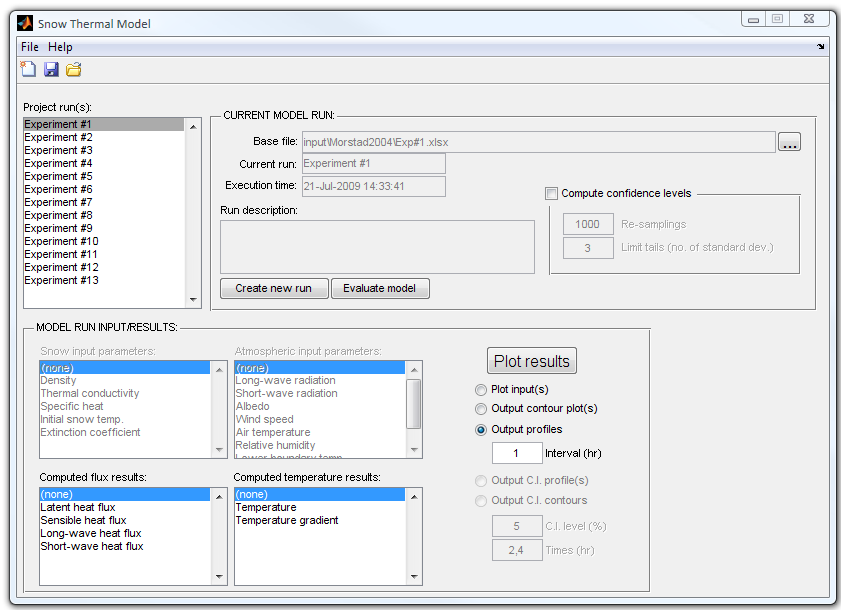
\includegraphics[width=\linewidth]{\cfolder /figures/gui.png}
\caption{Graphical user interface for implementing the snow thermal model.}
\label{TM:fig:gui}
\end{figure}

\subsection{Performing Model Runs}
The following briefly describes the basic steps of performing thermal model evaluations:
\begin{enumerate}
\item Select New Project from the file menu.
\item A prompt will appear that gives options regarding the Excel spreadsheet file to utilize.  Selecting New copies the template.xlsx file previously discussed to a file selected by the user.  Selecting Existing allows the user to select a previously created file.  In both cases the Excel file will open when the necessary actions are complete.
\item Modify and saved the Excel file created for the desired conditions, as detailed in Section \secref{TM:sec:spread}.
\item Return to the GUI application and type a name for the current run as well as a description. Also, if confidence levels are desired (see Section \ref{TM:sec:conf}) the Compute Confidence Levels option should be checked at this time.  The computation of the confidence levels can be extremely time consuming, so begin with a small number of re-samplings.
\item Press the Evaluate Model button on the GUI, this starts the model evaluations which may take several minutes depending on the computer and model inputs.  If confidence levels are being computed a window will appear showing the progress of the calculations.
\item When the run is complete it appears in the Project Run(s) menu on the left-side of the GUI.
\item Additional runs may be computed by selecting the Create New Run button and the Excel file may be changed by selecting the ``...'' button at the right-end of the Base File text. This same button will also open the associated Excel file when a model run is activated.  It is not necessary to create a new Excel file, but any changes made to the Excel file for additional model evaluations must be saved, these changes will not be stored and cannot not be recalled (this functionality may be available in future versions). Run names may be edited or runs may be deleted by right-clicking on the run in the Project Run(s) list.
\item After all the desired runs are completed the project should be saved by selecting Save Project from the File menu.
\end{enumerate}

\subsection{Graphing Results}
It is possible to create graphs of both the model inputs and outputs, this is done using the lower pane of the GUI shown in Figure \ref{TM:fig:gui}.  First, a model run must be selected in the Project Run(s) panel.  The graphs created share all of the functionallity of the graphs presented in Appendix \ref{apx:YCweather} (Section \secref{YC:sec:graphs}).

\subsubsection{Model Inputs}
The model inputs are graphed by selecting the Plot Input(s) radio button, this will cause the Snow and Atmospheric parameter lists to become activated. To create a graph simply select the desired item and press the Plot Results button. A graph will appear for each item selected. 

\subsubsection{Model Outputs}
Two different graph styles of model outputs are available: profiles and coutours.  Figure \ref{TM:fig:example} provides examples of the snowpack temperature graphed with each of the different methods.  When ploting profiles the interval, in hours, must also be set (e.g., 2 results in profiles being plotted every 2 hours). It is possible to graph a single profile directly from a contour plot, this is done be right-clicking on the contour where the profile is desired and the selecting either a vertical or horizontal profile. 

\begin{figure}[ht!]\centering
\subfloat[Temperature Profiles]{\includegraphics[width=0.47\linewidth]{\cfolder /figures/profiles.pdf}}\quad
\subfloat[Temperature Contours]{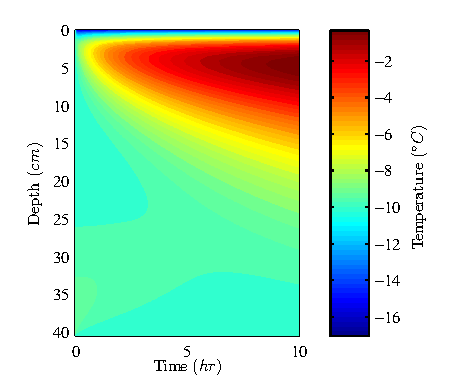
\includegraphics[width=0.47\linewidth]{\cfolder /figures/contours.pdf}}\quad
\caption{Example graphs of snowpack temperatures demonstrated the two graphing options available: (a) profiles and (b) contours.}
\label{TM:fig:example}
\end{figure}

In similar fashion, if confidence intervals were computed it is possible to graph these intervals using the Output C.I. Profiles or Contours radio buttons.  Figure \ref{TM:fig:ciexample} provides examples of temperature data plots with confidence level intervals.  Both the profiles and the contours require the confidence level to be specified by a scalar value (in percent) entered into the C.I. Level location.  When profiles are plotted the time(s) at which the profiles are desired must be specified in the Times (hr) location (e.g., 2 or 2, 4).  The confidence level contour graphs show the absolute value of the largest deviation from the mean value.

\begin{figure}[ht!]\centering
\subfloat[C.I. Profiles]{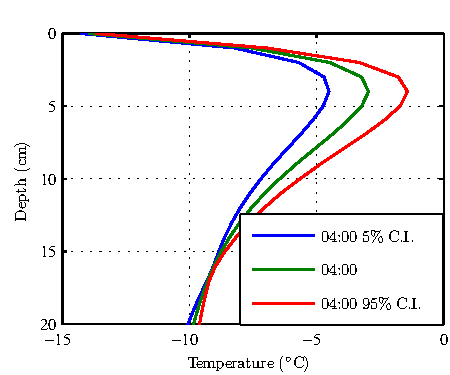
\includegraphics[width=0.47\linewidth]{\cfolder /figures/ciprofile.pdf}}\quad
\subfloat[C.I. Contours]{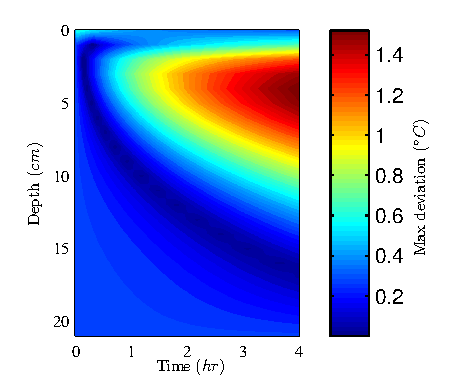
\includegraphics[width=0.47\linewidth]{\cfolder /figures/cicontour.pdf}}\quad
\caption{Example graphs of snowpack temperature demonstrated the two graphing options available for displaying confidence level intervals: (a) C.I. profiles and (b) C.I. contours.}
\label{TM:fig:ciexample}
\end{figure}

\subsection{Closing Remarks}
The information presented in this appendix explains the basic and advanced functionality of the thermal model developed for the work presented throughout this dissertation.  The details presented as well as the entire software package was developed to make the model easily accessible, thus please contact the author if more information is required.
